

\newtheorem{lemma}{Lemma}[subsection]
\newtheorem{thm}{Theorem}[subsection]
\newtheorem{defn}{Definition}[subsection]
\subsection{Hex}
Hex is a two-player turn-based game played on a rhombus-shaped board. Each player has a set of coloured hexagonal tiles and takes turns to place a tile in an empty cell on the board. For the purposes of this project, the first player is Red, and the second is Blue. The goal of the game is for a player to be the first to connect the two boundaries of the board corresponding to the player's colour.

\begin{figure}
    \centering
    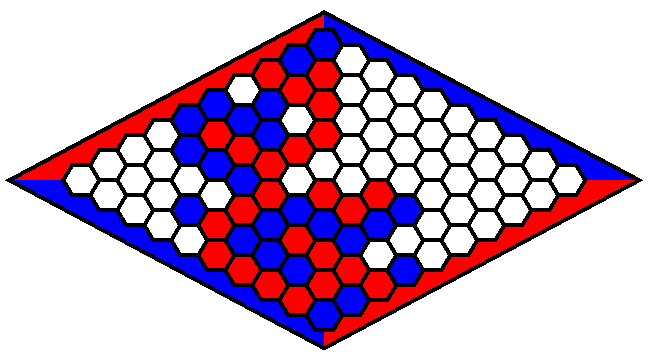
\includegraphics[scale = 0.4]{images/HEX_GAME.png}
    \caption{A finished game of Hex. Red has won.}
    \label{fig:hex_game}
\end{figure}

In Hex, there is a winning strategy for the first player (Red). This stems from a variety of results discussed below.

As explored and proven in \cite{GameOfHex}, it is impossible for the game to end in a draw:

\begin{lemma}If every tile of the Hex board is marked either blue or red, then there is either a blue path connecting blue boundaries, or a red path connecting red boundaries.\end{lemma}


We can also state another lemma, as described in \cite{MCTSHex}:

\begin{lemma}A player having an additional piece of their own colour on the board is never a disadvantage.\end{lemma}



From these two lemmas, we can deduce the following result as outlined in \cite{JNash}:



\begin{thm}There exists a winning strategy for the first player.\end{thm}

This can be proven by a move-stealing argument described in \cite{JNash}:


Since the game cannot end in a draw, there must be a winning strategy for one player. Suppose it is the second player that has this winning strategy. The first player can ``steal'' this strategy by playing a random move first (which can never be a disadvantage by Lemma 2.2) and ``becoming'' the second player (with an extra piece on the board). This player can then use the second player's winning strategy to win. Since this player was not the second player, the strategy is not a winning strategy, reaching a contradiction. Hence, the first player must own the winning strategy.

To help reduce the advantage the first player has due to this winning strategy, a rule can be implemented called the pie rule. This gives the second player the option to take the first player's move as their own on the first turn. The first player is therefore incentivized to make a ``neutral'' move, instead of a clearly advantageous one.

\subsection{Search Algorithms}
This report will focus on agents utilizing various algorithms (Monte Carlo tree search and minimax with alpha-beta pruning) as well as an algorithm more specific to Hex (H-Search \cite{HierarchicalHex}).


\subsubsection{Monte Carlo Tree Search}

Monte Carlo tree search (MCTS) is a best-first tree search guided by randomized game simulations \cite{MCTSHex}.

The algorithm starts with a tree consisting of just the root (which corresponds to the initial state) and repeatedly builds the tree by expanding nodes that have been selected to be promising. Each node in the tree has a corresponding game state.


MCTS is given in Algorithm \ref{MCTSAlgorithm}.











\begin{algorithm}
    \caption{Monte Carlo Tree Search}
    \label{MCTSAlgorithm}
    \begin{algorithmic}
        \Procedure{MCTS}{root : Node}
        \While{there is time left}
        \State node = root
        \While{node is not a leaf}
        \State node = node.mostPromisingChild()
        \EndWhile
        \State Expand node by adding all its children to the tree
        \State state = node.getState()
        \While{state is not terminal}
        \State update state with random move
        \EndWhile
        \State BackPropogate(node, state.winner)
        \EndWhile
        
        \EndProcedure
        
        \Procedure{backPropogate}{node, winner}
        \While{node is not null}
        \State increment node.state.visits 
        \If{node.state.player == winner}
        \State increment node.state.score by WIN\_SCORE
        \EndIf
        \State node = node.parent
        \EndWhile
        \EndProcedure
        
        
    \end{algorithmic}
    
\end{algorithm}




MCTS repeatedly executes four phases while there is time left. The four phases are:

\begin{enumerate}
    \item Selection
    \item Expansion
    \item Simulation
    \item Update
\end{enumerate}

In the selection phase, the algorithm traverses the tree to a leaf node in order to select a promising node. The exploration of new nodes and the exploitation of already considered nodes showing high value must be balanced. A way of doing this is to choose nodes at each level according to their UCT (Upper Confidence Bound 1 applied to trees) value, described in \cite{UCT2}:

\begin{center}
 \( UCT = X_{i, n_i} + \sqrt{\dfrac{2\ln p}{n_{i}}}\) 
 
\end{center}
 where:

\begin{itemize}
    \item $X_{i, n_i}$ is the empirical mean of the rewards for that node,
    \item $n_{i}$ is the number of times this node has been visited,
    \item $p$ is the number of times this node's parent has been visited.
\end{itemize}





In the expansion phase, we simply take the state corresponding to the node to be expanded and add a new child node to the tree for each possible next state. This builds the tree as we explore promising nodes, leading to the tree growing in the most promising areas.

In the simulation phase, we take the state corresponding to the promising node found in the selection phase, and carry out a randomized game from this state until termination. This is called a playout.

Using the result of the playout, we update the tree from the node to the root. If a state's last player was the winning player, we add a selected constant value to its score, as well as incrementing the visit counts appropriately.

\subsubsection{Minimax Algorithm with Alpha-Beta Pruning}


The minimax algorithm operates on a game tree, with the root node representing the initial state and each child of a node representing a possible next state. Each node in the game tree is implicitly labelled as either MAX or MIN: the root is labelled MAX, and a child of a MAX node is labelled MIN and vice-versa. The minimax algorithm is designed to determine the optimal next move for MAX \cite{AIModernApproach}.

In basic minimax each leaf node gives a score (the value of the game having played that path from root to leaf). Each node's value is updated with the maximum (or minimum) value of its children if the node is labelled MAX (or MIN). The best move is given by the child of the root with the highest value.

In reality, especially in games with large branch factors like Hex, game trees are usually too large for basic minimax. Alpha-beta pruning is an optimization technique to deal with this. We maintain two values, alpha and beta, that represent the best previously explored option on the path from the root for MAX and MIN respectively. Alpha is initially set to infinity and beta to negative infinity. We continually update alpha and beta to be the maximum and minimum values considered on the path to the root respectively. Whenever the minimum score that MAX is guaranteed becomes greater than the maximum score that MIN is guaranteed, MAX need not consider the children of this node. This is because it is impossible for this child's value to become the new maximum (or minimum) value.

Minimax with alpha-beta pruning can be seen in Algorithm \ref{alphabeta}.



\begin{algorithm}
    \caption{Minimax with Alpha-Beta Pruning}
    \label{alphabeta}
    \begin{algorithmic}
        \Procedure{min}{state, alpha, beta}
            \If{state.isFinished()}
                \State return evaluate(state)
            \Else 
                \State bestValue = $\infty$
                \For{child from state.getNextStates()}
                    \State value = MAX(child, alpha, beta)
                    \State bestValue = min(bestValue, value)
                    \State beta = min(beta, bestValue)
                    \If{beta $\leq$ alpha}
                        \State return bestValue
                    \EndIf
                \EndFor
            \EndIf
        
        \EndProcedure
        
        \Procedure{max}{state, alpha, beta}
            \If{state.isFinished()}
                \State return evaluate(state)
            \Else 
                \State bestValue = $-\infty$
                \For{child from state.getNextStates()}
                    \State value = MIN(child, alpha, beta)
                    \State bestValue = min(bestValue, value)
                    \State beta = min(beta, bestValue)
                    \If{beta $\leq$ alpha}
                        \State return bestValue
                    \EndIf
                \EndFor
            \EndIf
        
        \EndProcedure
        
        
    \end{algorithmic}
    
\end{algorithm}



The most notable improvement from alpha-beta pruning occurs when the best moves are considered first. This is because we form a tighter bound using alpha and beta, and can subsequently prune more nodes.

In large games the game tree is still too large, even with pruning. A solution to this is to use a heuristic at a set depth, instead of traversing the game tree to completion. This heuristic can evaluate a state, assigning it a quantitative value, which is then treated as a leaf. 



\subsubsection{H-Search}



The main difficulty in constructing a good heuristic for Hex is that strong board positions are subtle: it is not easy to assign a quantitative value to how good a board is for a particular player since its strength is made up of a variety of factors. 

A solution to this is to use an algorithm concerned specifically with the analysis of cell positions on a Hex board. This algorithm considers a player's tiles on the board, and decides their potential for connection.

H-Search is an algorithm introduced in \cite{HierarchicalHex} which aims to complete this analysis for Hex boards.

In this section we will consider boards from Red's point of view.

As described in \cite{HierarchicalHex}, we first introduce the idea of sub-games and carriers:


\begin{defn} \normalfont Let x and y be two different cells, and let A be a set of empty cells of a given
position. We assume that x $\notin$ A and y $\notin$ A. Consider the triplet (x, A, y) as a sub-game,
where Red tries to connect cells x and y with a chain of red pieces, Blue tries to
prevent it, and both players can put their pieces only in cells of A. We then define x and y
as ends of the sub-game, and A as its carrier \cite{HierarchicalHex}.\end{defn}



As further described in \cite{HierarchicalHex}, we can then go on to define properties of sub-games:

\begin{defn} \normalfont A sub-game is a virtual connection if and only if Red has a winning strategy [for the sub-game] even if
Blue moves first \cite{HierarchicalHex}.\end{defn}

\begin{defn} \normalfont A sub-game is a virtual semi-connection if and only if Red has a winning strategy
moving first, and does not have one if he moves second. \cite{HierarchicalHex}\end{defn}

A \textit{two-bridge} is a special case of virtual connection where the ends are separate by two empty cells each neighbouring both ends.



A virtual connection (x, A, y) is minimal if and only if there is no other virtual connection (x, B, y) such that B $\subset$ A \cite{HierarchicalHex}.

We can now introduce deduction rules to be able to combine sub-games into larger sub-games. 

\textbf{AND Deduction Rule}, as described in \cite{HierarchicalHex}:

\textit{Let sub-games (x, A, u) and (u, B, y) be two virtual
connections, with common end u and different ends x $\neq$ y. We assume that x $\notin$ B, y $\notin$ A,
and A $\cap$ B = $\emptyset$.}
\begin{itemize}
    \item \textit{If u is red, then the sub-game (x, A $\cup$ B, y) is a virtual connection.}
    \item \textit{If u is empty, then the sub-game (x, A $\cup$ \{u\} $\cup$ B, y) is a virtual semi-connection.}
\end{itemize}



\begin{figure}
    \centering
    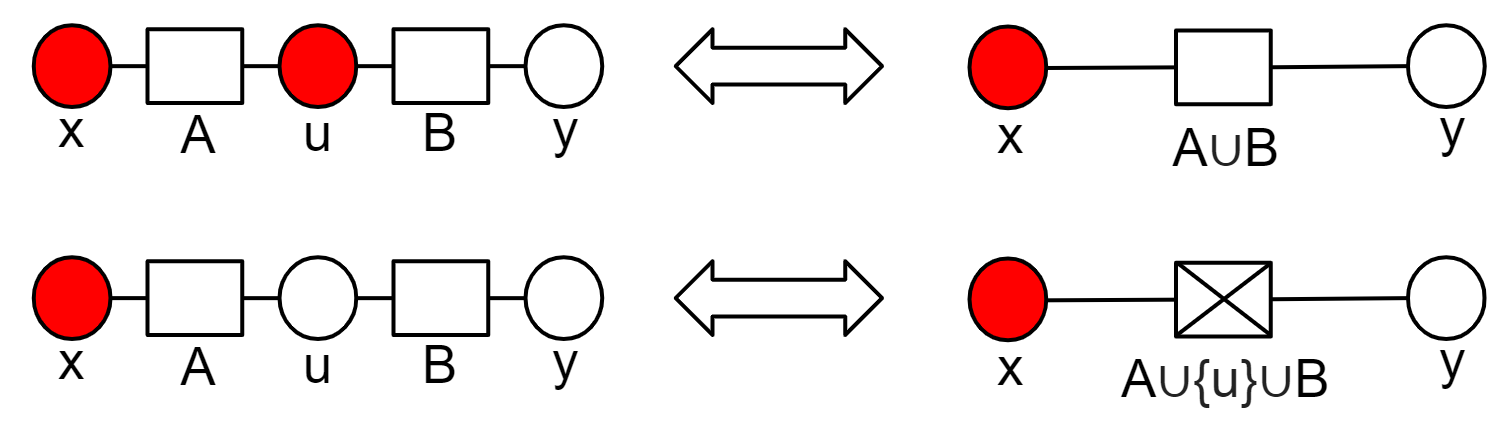
\includegraphics[scale = 0.2]{images/AND_deduction.png}
    \caption{The \textbf{AND} deduction rules. }
    \label{fig:and_deduction}
\end{figure}


\textbf{OR Deduction Rule}, as described in \cite{HierarchicalHex}:

\textit{Let sub-games (x, $A_k$,y) (k = 1, 2,...,n, for n $>$ 1) with common ends x and y be virtual semi-connections. If}

$\bigcap\limits_{k=1}^{n} A_{k} = \emptyset$

\textit{then the sub-game (x, A, y), where}

$A = \bigcup\limits_{k=1}^{n} A_{k}$

\textit{is a virtual connection.}
\newline
\newline

\begin{figure}
    \centering
    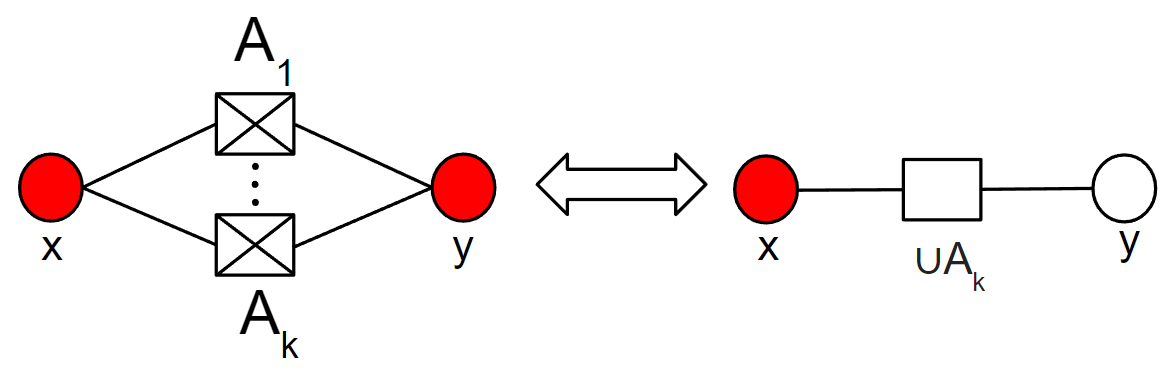
\includegraphics[scale = 0.26]{images/OR_deduction.png}
    \caption{The \textbf{OR} deduction rule.}
    \label{fig:or_deduction}
\end{figure}

Proofs of these deduction rules are found in \cite{HierarchicalHex}. The \textbf{AND} and \textbf{OR} rules can be seen diagrammatically in Figures \ref{fig:and_deduction} and \ref{fig:or_deduction} respectively. Circles filled with colour \textit{c} represent a cell with a tile of colour \textit{c} in it (or an empty cell if no colour) and blank rectangles and crossed rectangles represent carriers in virtual connections and virtual semi-connections respectively.



\begin{figure}
\centering
\begin{subfigure}{.5\textwidth}
  \centering
  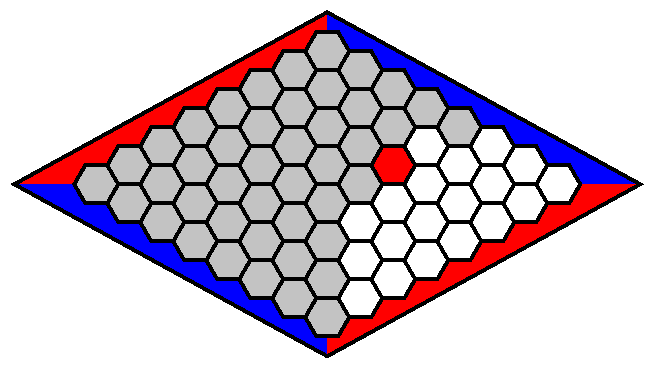
\includegraphics[width=0.94\linewidth]{images/BIG_VC.png}
  \caption{An edge virtual connection.}
  \label{fig:sub1}
\end{subfigure}%
\begin{subfigure}{.5\textwidth}
  \centering
  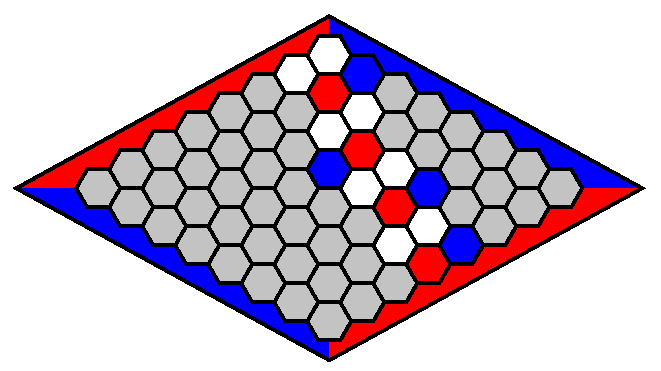
\includegraphics[width=0.95\linewidth]{images/SMALL_VC.png}
  \caption{Multiple \textit{two-bridges}.}
  \label{fig:sub2}
\end{subfigure}
\caption{Examples of virtual connections. The carriers of the virtual connections are represented by the white cells.}
\label{fig:test}
\end{figure}



We can now introduce the H-Search algorithm to build up virtual connections from a small initial set of virtual connections. We call the initial virtual connections the \textit{first generation} of virtual connections \cite{HierarchicalHex}, and merge them using the deduction rules to generate the \textit{second generation}. We can then repeat this process until we have formed a virtual connection between the player's boundaries, or we stop generating new virtual connections. The initial set of virtual connections is usually pairs of neighbouring cells.

It is important to note that H-Search is not complete \cite{HierarchicalHex}, so there are some virtual connections that cannot be found. 

Pseudo-code of the H-Search algorithm, as presented in \cite{HierarchicalHex}, can be seen in Algorithm \ref{hsearchalgorithm}.

\begin{algorithm}
    \caption{H-Search}
    \label{hsearchalgorithm}
    \begin{algorithmic}
        \Procedure{Search}{}
            \State Initiate G to set of red and empty cells
            \For{$g1, g2 \in G$}
                
                \State $C(g1,g2) = \emptyset$ if g1 and g2 are not nearest neighbours
                \State $C(g1,g2) = \{\emptyset\}$ if g1 and g2 are nearest neighbours
                \State $SC(g1,g2) = \emptyset$
            \EndFor
            \While{there is at least one new virtual connection}
                \For{$g \in G$}
                    \For{$g1, g2 \in G$ such that: \newline\indent\indent\indent\indent$g1 \neq g2$,\newline\indent\indent\indent\indent at least one of the lists C(g1, g) or C(g2, g) contains at\newline\indent\indent\indent\indent least one new carrier.\newline\indent\indent\indent\indent If g is red then, additionally, g1 and g2 should be both \newline\indent\indent\indent\indent empty.}
                        \For{$c1 \in C(g1, g)$ and $c2 \in C(g2, g)$ such that: \newline\indent\indent\indent\indent\indent At least one of the carriers c1 or c2 is new,\newline\indent\indent\indent\indent\indent $c1 \cap c2 = \emptyset$ \newline\indent\indent\indent\indent\indent $g1 \notin c2$ and $g2 \notin c1$}
                        
                            \If{g is red}
                                \State{$c = c1 \cup c2$}
                                \State{Update C(g1, g2) with c}
                            \Else
                                \State{$sc = c1 \cup g \cup c2$}
                                \State{Update SC(g1, g2) with sc}
                                \If{last update is successful}
                                    \State{ApplyOrRule(C(g1, g2), SC(g1, g2)-sc, sc, sc)}
                                \EndIf
                            \EndIf
                        \EndFor
                    \EndFor
                \EndFor
                   
            \EndWhile
        
        \EndProcedure
        \Procedure{ApplyOrRule}{C, SC, union, intersection}
            \For{$scl \in SC$}
                \State{$ul = union \cup scl$}
                \State{$il = intersection \cap scl$}
                \If{$il = \emptyset$}
                    \State{Update C with ul}
                \Else
                    \State{ApplyOrRule(C, SC-scl, ul, il)}
                \EndIf
            \EndFor
        \EndProcedure
  
        
        
    \end{algorithmic}
    
\end{algorithm}



\subsubsection{Ford-Fulkerson Method}

The Ford-Fulkerson method is a method to compute the maximum flow possible through a flow network.

A flow network is defined as a directed graph $G= (V,E)$ with a non-negative capacity function $c: E \to \mathbb{R}$ \cite{networkflow} which indicates the maximum amount of flow that can be sent along one particular edge. Graph $G$ must contain a source $s$ and a sink $t$ in $V$, indicating the start and end of the flow.

A network flow is defined as a function $f: E \to \mathbb{R}$ that satisfies the following constraints:

\begin{itemize}
    \item $\forall(u,v) \in E, \;\;\; f(u,v) \leq c(u,v)$  (capacity constraint)  \cite{networkflow},
    \item $\forall(u,v) \in E, \;\;\; f(u,v) \geq 0$.
\end{itemize}

The method repeatedly finds augmenting paths. An augmenting path is a path from source to sink with available capacity. Once no more augmenting paths can be found, we have found the maximal flow.

We can find augmenting paths through breadth-first search over the network. In this case, the method is referred to as the Edmonds-Karp algorithm \cite{networkflow}.


